\chapterimage{chapter_head_2.pdf} % Chapter heading image

\chapter{Eletricidade para o Ensino Médio}
\subsection{Associação de resistores em série}\index{Resistores em série}

Considere a imagem obtida pelo simulador TinkerCAD.

\begin{figure}[H]
	\caption{Simulação de resistores em série}
	\begin{center}
		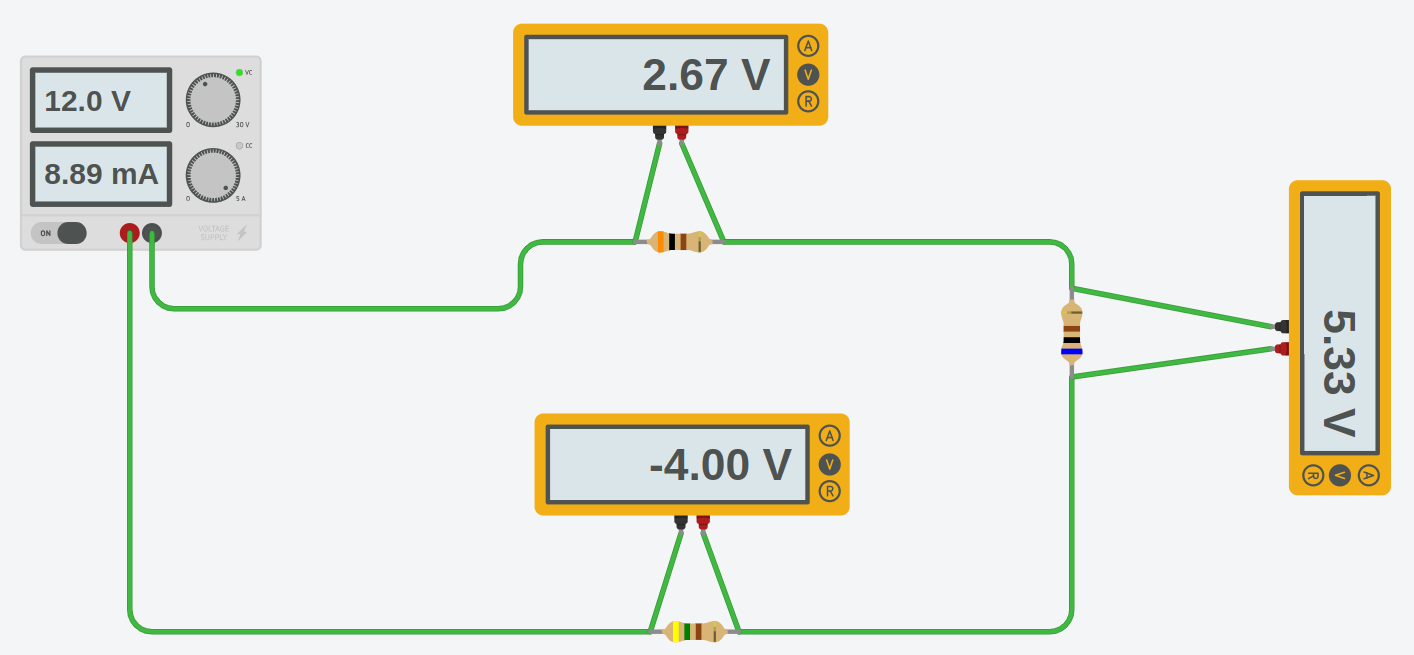
\includegraphics[width=\linewidth]{Pictures/FISICA_EM/ELETRICIDADE/resistores_serie.png}
	\end{center}
	\label{fig:funcao_linear}
	%\vspace{-1cm}
	%\begin{center}
	%\makebox[\width]{Legenda}
	%\end{center}
	\hspace{1.5cm}\makebox[\width]{Fonte: Próprio autor.}
\end{figure}


1 - Por que o sinal de Voltagem no resistor 3 apresenta um valor negativo?
R: O valor negativo no multímetro acontece ao medir a tensão em um resistor porque as pontas de prova do multímetro foram colocadas invertidas, ou seja, o \textit{polo positivo} foi colocado na parte \textit{negativa} e vice-versa.

2 - Calcule as resistências dos resistores baseado no projeto do TinkerCAD.

R: O primeiro passo para ser verificado é se a associção de resistores no circuito é em série ou em paralelo.
Como pode ser visto, os resistores estão todos conectados no mesmo fio, então a associação desses resistores é em SÉRIE!

Em um circuito em série, temos:
\begin{itemize}
    \item{a corrente elétrica no circuito é constante}
    \item{a tensão em cada resistor, varia}
\end{itemize}

Através dos dados obtidos pelo simulador, é possível verificar que a corrente elétrica é de $8,89 \text{mA}$.

Pela lei de Ohm, temos:

\begin{ceqn}
    \begin{align*}
        U =& R \cdot i \\
    \end{align*}
\end{ceqn}

Como é fornecido os valores de corrente elétrica e tensão em cada resistor, basta isolar $R$ na equação acima e obtemos uma relação geral para determinar a resistência de cada resistor, assim:

\begin{ceqn}
    \begin{align*}
        U =& R \cdot i \\
        R =& \frac{U}{i} \\
    \end{align*}
\end{ceqn}

Antes de efetuarmos os cálculos para a resistência de cada resistor será interessante passar a corrente elétrica de mA para A fazendo o valor em mA dividido por 1000, assim:

\begin{ceqn}
    \begin{align*}
        i = \frac{8,89 [\text{mA}]}{1000} \\
        i = 0,0089 [\text{A}] \\
    \end{align*}
\end{ceqn}

Para o resistor 1, temos:

\begin{ceqn}
    \begin{align*}
        R_1 =& \frac{U_1}{i} \\
        R_1 =& \frac{2,67}{0,0089} \\
        R_1 =& 300 \Omega \\
    \end{align*}
\end{ceqn}

Para o resistor 2, temos:

\begin{ceqn}
    \begin{align*}
        R_2 =& \frac{U_2}{i} \\
        R_2 =& \frac{5,33}{0,0089} \\
        R_2 =& 598,87\Omega \\
        R_2 \approx & 600 \Omega \\
    \end{align*}
\end{ceqn}

Para o resistor 3, temos:

\begin{ceqn}
    \begin{align*}
        R_3 =& \frac{U_3}{i} \\
        R_3 =& \frac{4,00}{0,0089} \\
        R_3 =& 449,4\Omega \\
        R_3 \approx & 450 \Omega \\
    \end{align*}
\end{ceqn}


\subsection{Associação de resistores em paralelo}\index{Resistores em paralelo}

Os resistores associados paralelamente possuem duas características:

\begin{itemize}
    \item{A voltagem nos resistores são iguais a voltagem da fonte}
    \item{A corrente elétrica em cada resistor muda}
\end{itemize}

A resistência equivalente a uma quantidade "n" de resistores em paralelo pode ser determinada como:

\begin{ceqn}
    \begin{align*}
        \frac{1}{R_{\text{eq}}} = \sum_{i=1}^{n} \frac{1}{R_i}
    \end{align*}
\end{ceqn}


No nosso exemplo da aula temos dois resistores em paralelo; um com $6 \Omega$ e outro com $3 \Omega$.

Substituindo na fórmula, obteremos:

\begin{ceqn}
    \begin{align*}
        \frac{1}{R_{\text{eq}}} =& \frac{1}{6} + \frac{1}{3} \\
        =& 0,17+ 0,33 \\
        \frac{1}{R_{\text{eq}}} =& 0,5 \\
        R_{\text{eq}} =& \frac{1}{0,5} \\
        R_{\text{eq}} =& 2 \Omega \\
    \end{align*}
\end{ceqn}

Logo, a associação dos resistores em paralelo resultou em um resistor equivalente de $2 \Omega$. 

Esse resistor equivalente, agora, está em série com o outro resistor de $3 \Omega$. Desse modo, a resistência total do circuito será de $2 \Omega + 3 \Omega = 5 \Omega$

pela Primeira Lei de Ohm, é sabido que $U = R \cdot i$. O valor da tensão da fonte é igual a $60 \text{V}$, assim, substituindo os valores conhecidos, será possível calcular a corrente elétrica, como segue:


\begin{ceqn}
    \begin{align*}
        U =& R \cdot i \\
        i =& \frac{U}{R} \\
        i =& \frac{60 \text{V}}{5 \Omega} \\
        i =& 12 \text{A} \\
    \end{align*}
\end{ceqn}


Segunda lei de Ohm

\begin{ceqn}
    \begin{align*}
        R =& \rho \cdot \frac{L}{A}
    \end{align*}
\end{ceqn}



\begin{ceqn}
    \begin{align*}
        R =& \rho \cdot \frac{L}{A} \\
        =& 17 [\Omega \cdot \text{nm}] \cdot \frac{0,5 [\text{nm}]}{0,05 [\text{nm}^2]}
    \end{align*}
\end{ceqn}

Equação de Clapeyron
\begin{ceqn}
    \begin{align*}
        p \cdot V =& n \cdot R \cdot T \\
        2 \text{atm} \cdot 2 \text{m}^3 =& n \cdot 0,0000821 \cdot 100 \text{K} \\
        4 =& n \cdot {0,00821} \\
        n =& \frac{4}{0,00821} \\
        n \approx& 487,2 \text{mols}\\
    \end{align*}
\end{ceqn}


